\documentclass{minimal}
\usepackage{tikz}
\usetikzlibrary{arrows,positioning} 

\begin{document}

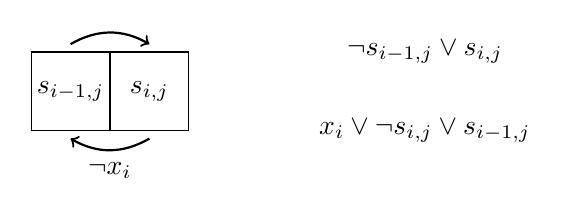
\begin{tikzpicture}[node distance=1cm, auto,]

\coordinate (A) at (0.5,1.1);
\coordinate (B) at (1.5,1.1);
\coordinate (C) at (0.5,-0.1);
\coordinate (D) at (1.5,-0.1);

\draw (0, 0) rectangle (1, 1);
\draw (1, 0) rectangle (2, 1);
\draw[->,thick] (A) to [bend left] (B);
\draw[->,thick] (D) to [bend left] (C);


\node at (0.5,0.5) {$s_{i-1,j}$};
\node at (1.5,0.5) {$s_{i,j}$};
%\node at (1,1.5) {test};
\node at (1,-0.5) {$\neg x_i$};

\node at (5,1) {$\neg s_{i-1,j} \vee s_{i,j}$};
\node at (5,0) {$x_{i} \vee \neg s_{i,j} \vee s_{i-1,j}$};

\end{tikzpicture}

\vspace{1cm}

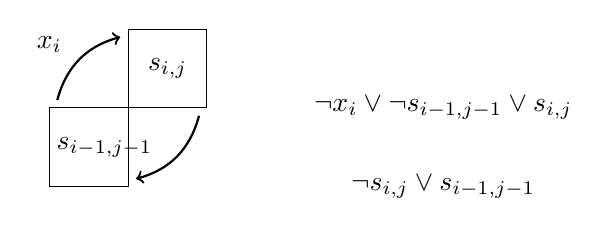
\begin{tikzpicture}[node distance=1cm, auto,]

\coordinate (A) at (0.1,1.1);
\coordinate (B) at (0.9,1.9);
\coordinate (C) at (1.1,0.1);
\coordinate (D) at (1.9,0.9);

\draw (0, 0) rectangle (1, 1);
\draw (1, 1) rectangle (2, 2);
\draw[->,thick] (A) to [bend left] (B);
\draw[->,thick] (D) to [bend left] (C);

\node at (0.7,0.5) {$s_{i-1,j-1}$};
\node at (1.5,1.5) {$s_{i,j}$};
\node at (0,1.8) {$x_i$};
%\node at (2,0) {test};

\node at (5,1) {$\neg x_{i} \vee \neg s_{i-1,j-1} \vee s_{i,j}$};
\node at (5,0) {$\neg s_{i,j} \vee s_{i-1,j-1}$};

\end{tikzpicture}

\vspace{1cm}

\begin{tikzpicture}[node distance=1cm, auto,]

\coordinate (A) at (0.5,1.1);
\coordinate (B) at (2.9,3.5);

\draw (0, 0) rectangle (1, 1);
\draw (3, 3) rectangle (4, 4);
\draw[->,thick] (B) to [bend right] (A);

\draw[dashed] (3.5,0.5) -- (3.5,3);
\draw[dashed] (1.5,0.5) -- (3.5,0.5);

\node at (0.7,0.5) {$s_{i-q,j-u}$};
\node at (3.5,3.5) {$s_{i,j}$};

\node at (4,2) {$u$};
\node at (2.5,0) {$q$};

\node at (7,2) {$\neg s_{i,j} \vee s_{i-q,j-u}$};

\end{tikzpicture}

\end{document}
